\section{Resultados y Discusi\'on: PageRank}
\subsection{Experimentos sobre la convergencia de PageRank}

\subsubsection{Experimento 1}
\par El primer experimento consiste en aumentar la cantidad de p\'aginas del grafo, manteniendo constante la cantidad (en particular, 4) de links que salen de cada una de \'estas.
En las figuras \ref{fig:grafo1s10}, \ref{fig:grafo1s50}, \ref{fig:grafo1s100}, y \ref{fig:grafo1s250} se pueden ver graficados algunos de los inputs.
Cabe destacar que los links est\'an relativamente distribuidos a lo largo del grafo: todas las p\'aginas tienen la misma cantidad de links salientes, y si bien la cantidad de links
entrantes puede variar (ya que esto fue generado aleatoriamente en el input), estad\'isticamente esta magnitud deber\'ia ser homog\'enea.
Los colores no poseen ning\'un significado y s\'olo son incluidos por claridad (se vuelve d\'ificil comprender los grafos monocromos).

\FloatBarrier
\begin{figure}[ht]
\subfigure[Grafo del experimento 1, para un tama\~no de 10 p\'aginas]{
	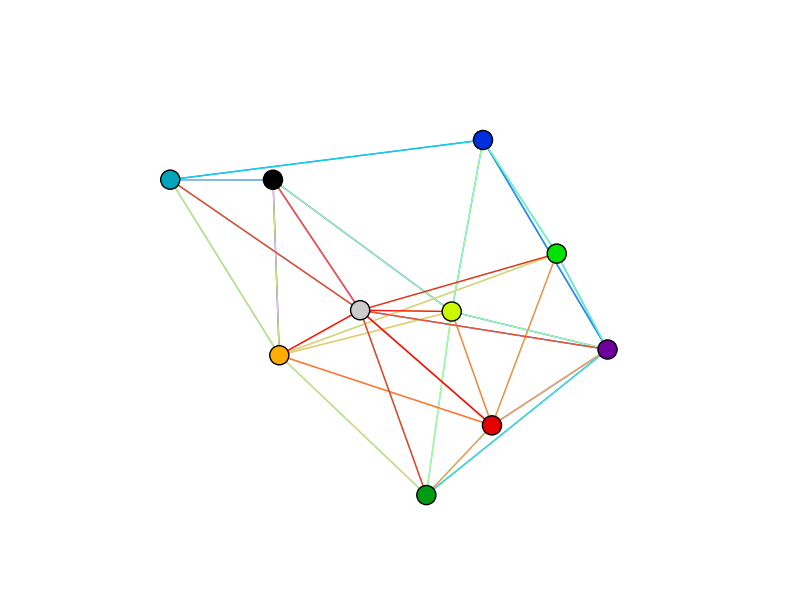
\includegraphics[width=0.45\columnwidth]{imagenes/exp1s10}
	\label{fig:grafo1s10}
}
\qquad
\subfigure[Grafo del experimento 1, para un tama\~no de 50 p\'aginas]{
	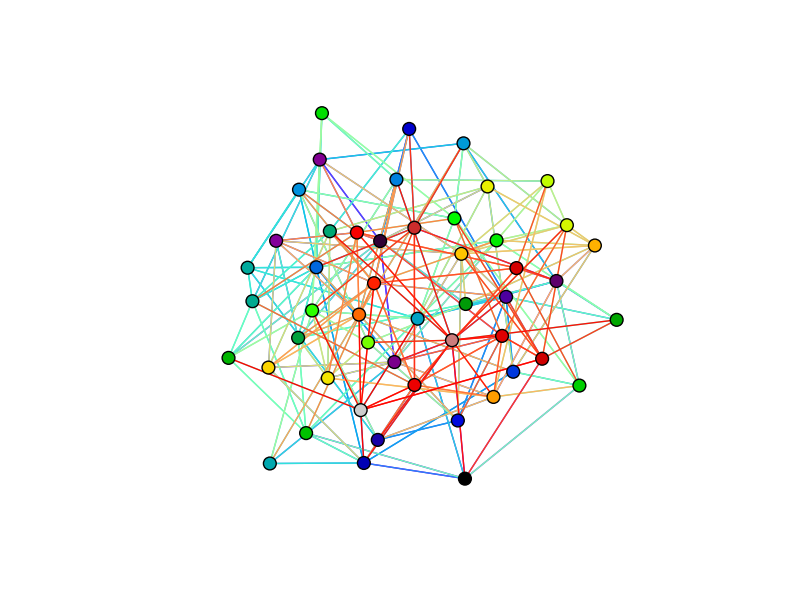
\includegraphics[width=0.45\columnwidth]{imagenes/exp1s50}
	\label{fig:grafo1s50}
}
\end{figure}

\begin{figure}[ht]
\subfigure[Grafo del experimento 1, para un tama\~no de 100 p\'aginas]{
	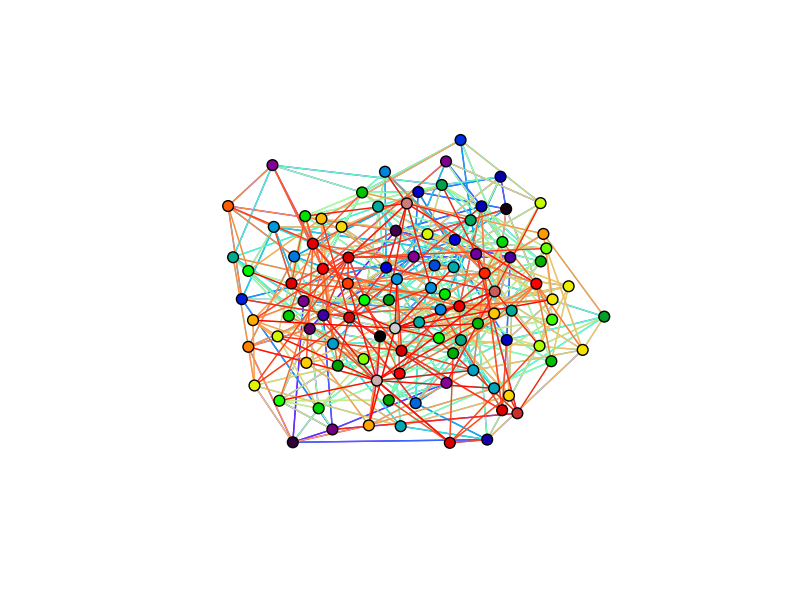
\includegraphics[width=0.45\columnwidth]{imagenes/exp1s100}
	\label{fig:grafo1s100}
}
\qquad
\subfigure[Grafo del experimento 1, para un tama\~no de 250 p\'aginas]{
	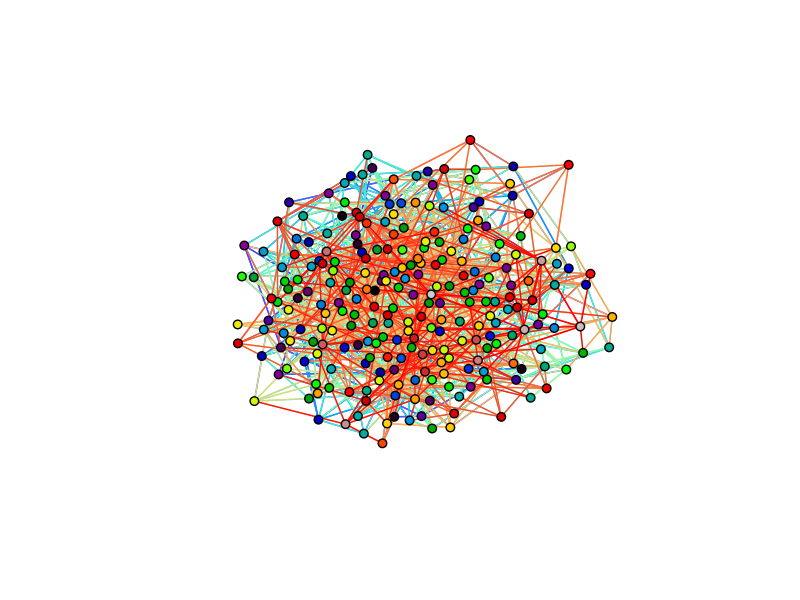
\includegraphics[width=0.45\columnwidth]{imagenes/exp1s250}
	\label{fig:grafo1s250}
}
\end{figure}


\FloatBarrier

\subsubsection{Experimento 2}
\par El experimento 2 es similar al primero: se observa c\'omo var\'ia el tiempo de ejecuci\'on al variar la cantidad de elementos no-nulos de la matriz de Markov.
La diferencia reside en modificar la cantidad de links que salen de cada p\'agina, manteniendo constante la cantidad total de p\'aginas -en particular, 1000 p\'aginas- 
(es decir, al rev\'es que en el experimento 1).
Si bien ambos experimentos miden lo mismo, el primero lo hace manteniendo de cierta forma la esparsidad de la matriz, mientras que el segundo lo hace modific\'andola.
En las figuras \ref{fig:grafo2s10}, \ref{fig:grafo2s50}, y \ref{fig:grafo2s100} se pueden ver graficados algunos de los inputs.
Cabe destacar como el grafo se vuelve paulatinamente m\'as interconectado.

\FloatBarrier

\begin{figure}[ht]
\subfigure[Grafo del experimento 2, para 1 link saliente por p\'agina]{
	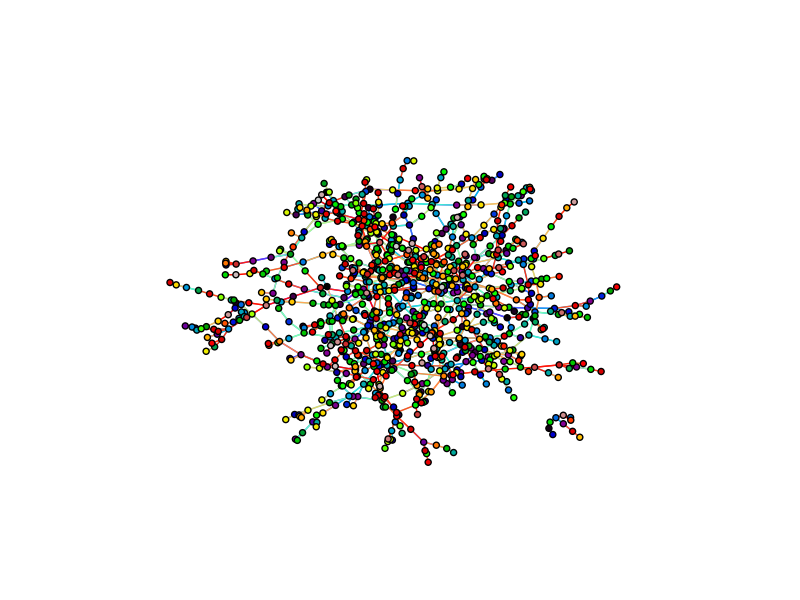
\includegraphics[width=0.45\columnwidth]{imagenes/exp2s10}
	\label{fig:grafo2s10}
}
\qquad
\subfigure[Grafo del experimento 2, para 2 links salientes por p\'agina]{
	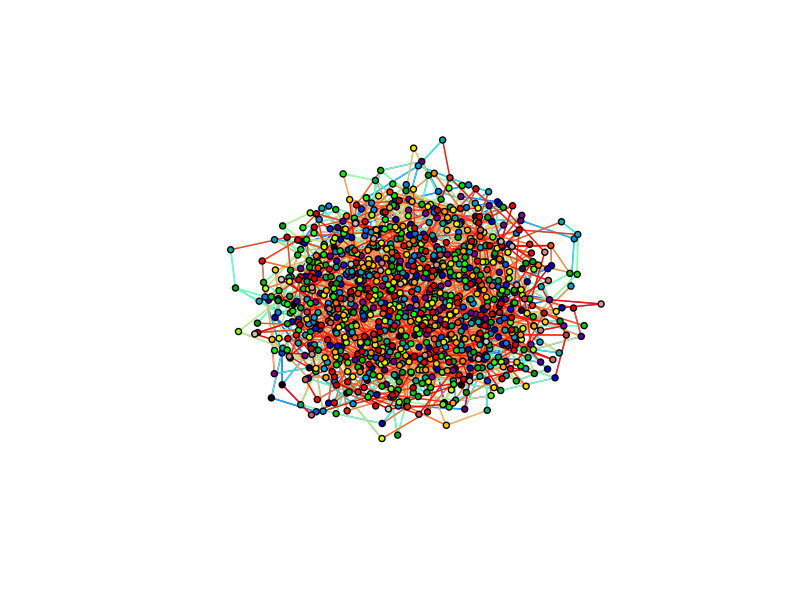
\includegraphics[width=0.45\columnwidth]{imagenes/exp2s50}
	\label{fig:grafo2s50}
}
\end{figure}

\begin{figure}[ht]
\subfigure[Grafo del experimento 2, para 4 links salientes por p\'agina]{
	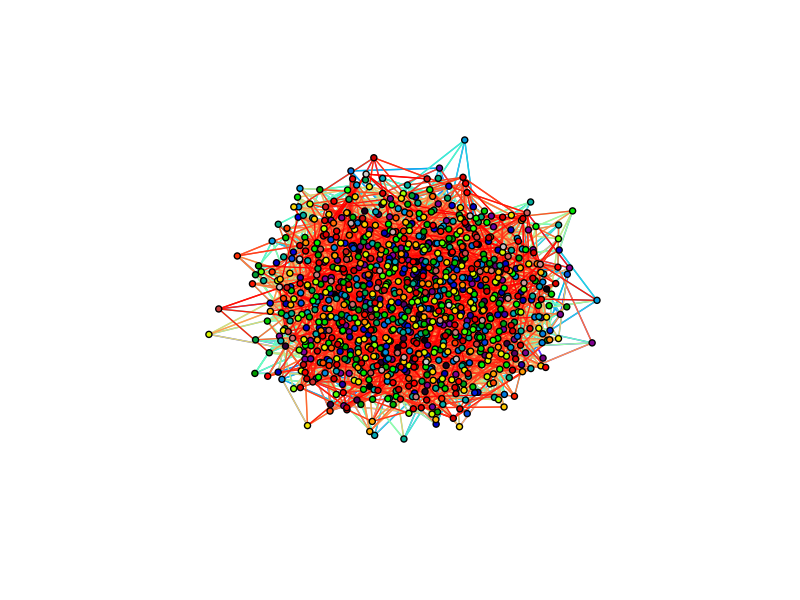
\includegraphics[width=0.45\columnwidth]{imagenes/exp2s100}
	\label{fig:grafo2s100}
}
\end{figure}


\FloatBarrier

\subsubsection{Resultados de los Experimentos 1 y 2}
\par En las figuras \ref{fig:res1}, y \ref{fig:res1zoom} se pueden observar los resultados del experimento 1 (la segunda figura muestra s\'olo los primeros 4 valores, por claridad).
En la figura \ref{fig:res2}, los del experimento 2.
Para permitirnos mejor comparar los resultados de ambos experimentos, se han incluido los dos juntos en la figura \ref{fig:res1y2} 
(la variable dependiente en este caso representa la cantidad de elementos no-nulos de la matriz).

\FloatBarrier
\begin{figure}[ht]
\begin{center}
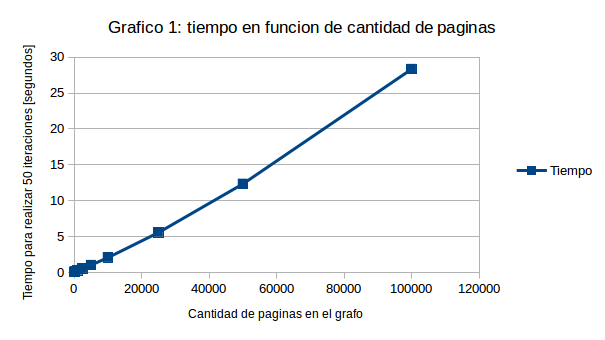
\includegraphics[width=0.8\columnwidth]{imagenes/graf1}
\caption{Resultado del experimento 1}
\label{fig:res1}
\end{center}
\end{figure}

\begin{figure}[ht]
\begin{center}
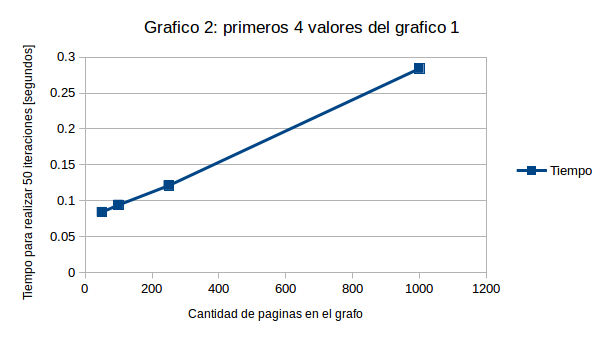
\includegraphics[width=0.8\columnwidth]{imagenes/graf2}
\caption{Resultado del experimento 1, primeros 4 valores}
\label{fig:res1zoom}
\end{center}
\end{figure}

\begin{figure}[ht]
\begin{center}
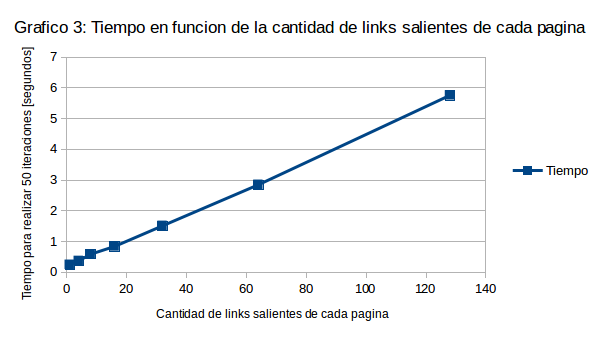
\includegraphics[width=0.8\columnwidth]{imagenes/graf3}
\caption{Resultado del experimento 2}
\label{fig:res2}
\end{center}
\end{figure}

\begin{figure}[ht]
\begin{center}
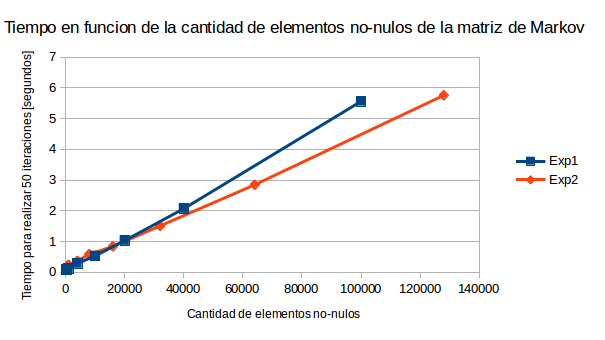
\includegraphics[width=0.8\columnwidth]{imagenes/graf6}
\caption{Resultado del experimento 1 y 2, juntos}
\label{fig:res1y2}
\end{center}
\end{figure}
\FloatBarrier

\par Se puede ver que los resultados de ambos experimentos describen curvas similares, pero la pendiente del primero es m\'as dr\'astica.
Esto es esperable, ya que si bien cada iteraci\'on del m\'etodo de la potencia depende linealmente de la cantidad de elementos no-nulos de la matriz,
tambi\'en depende linealmente de la cantidad de p\'aginas (el tama\~no de los vectores uniformes utilizados est\'a dado por la cantidad de nodos en el grafo, es decir de sitios en la red).

\subsubsection{Experimento 3}
\par Para el experimento 3, se medir\'a el tiempo de ejecuci\'on para una misma entrada (con 10000 p\'aginas y 4 links salientes de cada una), variando el par\'ametro \textit{''c''}.
\par Sabemos que \textit{''c''} es igual al módulo del segundo autovalor de la matriz
(como se encuentra demostrado en el paper \emph{The Second Eigenvalue of the Google Matrix}$^{\cite{Kamvar2}}$ de Kamvar y Haveliwala). Como vimos en la introducción teórica, el m\'etodo de la potencia trata obtener el primer autovalor al eliminar al resto en la combinaci\'on lineal, haciéndolos converger a 0 aplicando potenciación ya que son menores que 1. 
Cuanto mayor sea el $c$, y por ende, más cercano a 1 sea el módulo de $\lambda_2$, se espera que requiera de m\'as iteraciones para que $\lambda_2$ converja a 0 (en términos del algoritmo, que sea menor que $\varepsilon$).

\subsubsection{Experimento 4}
\par En el experimento 4, mediremos el tiempo de ejecuci\'on para la una misma entrada (id\'entica a la del tercer experimento) al variar el par\'ametro $\varepsilon$.

\subsubsection{Resultados de los Experimentos 3 y 4}
\par En las figuras \ref{fig:res3} y \ref{fig:res4} se encuentran los resultados de los experimentos 3 y 4, respectivamente.
Cabe destacar que la escala utilizada para el par\'ametro $\varepsilon$ en la figura \ref{fig:res4} es logar\'itmica.
\FloatBarrier

\begin{figure}[ht]
\begin{center}
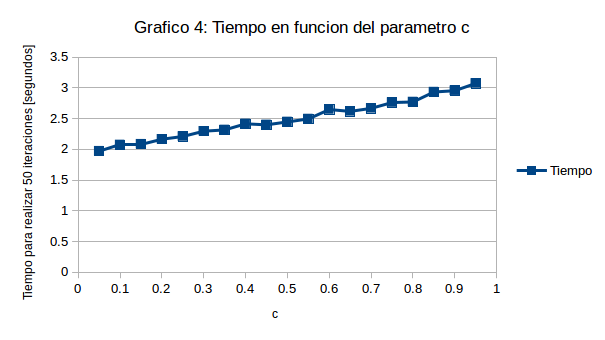
\includegraphics[width=0.8\columnwidth]{imagenes/graf4}
\caption{Resultado del experimento 3}
\label{fig:res3}
\end{center}
\end{figure}

\begin{figure}[ht]
\begin{center}
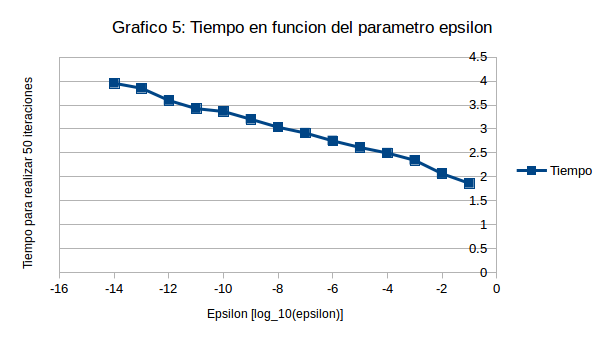
\includegraphics[width=0.8\columnwidth]{imagenes/graf5}
\caption{Resultado del experimento 4}
\label{fig:res4}
\end{center}
\end{figure}
\FloatBarrier

\par Se ve claramente que al aumentar el par\'ametro \textit{''c''} aumenta el tiempo de ejecución para computar el autovector principal. Lo mismo sucede al decrementar el $\varepsilon$, ya que disminuimos el margen que tomamos para traducir que los $|\lambda|$ convergen a 0.
\par Esto puede ser \'util si se desea realizar PageRank con un \textit{''c''} alto pero se debe calcular en un tiempo bajo, se puede incrementar $\varepsilon$ (aunque se pierda un poco de presici\'on).
\par Una observación es importante es que a pesar de que al disminuir el par\'ametro \textit{''c''} el algoritmo se vuelve más rápido, aumenta la probabilidad de teletransportación y esto puede dar lugar a páginas con un alto ranking injusto. (ver Experimento 3 de la sección de resultados para Competencias Deportivas).

\subsection{Experimentos sobre la eficacia de In-Deg, PageRank y PageRank con personalizaci\'on}
\subsubsection{Experimento 5}
\par El experimento 5 (y el 6) buscan comparar la eficiencia de PageRank e In-Deg en distintos escenarios.
Son dos de los ejemplos que m\'as comunmente se utilizan para detallar las ventajas de PageRank, y nuestra intenci\'on es comprobar que el algoritmo es efectivamente superior en estos casos.
\par En el caso del 5, la entrada consiste en un grafo donde hay una p\'agina ''central'' (como ser\'ian Google, Facebook, Wikipedia y dem\'as) a la que apunta la mayor\'ia de las p\'aginas.
El resto de las p\'aginas se distribuyen uniformemente (es decir, mediante una variable aleatoria uniforme) los links salientes.
La idea es que la p\'agina m\'as importante deber\'ia ser la central, y las que la siguen en prioridad deber\'ian ser p\'aginas apuntadas por \'esta.
En la figura \ref{fig:grafo5} se puede observar representado el input.

\FloatBarrier
\begin{figure}[ht]
\begin{center}
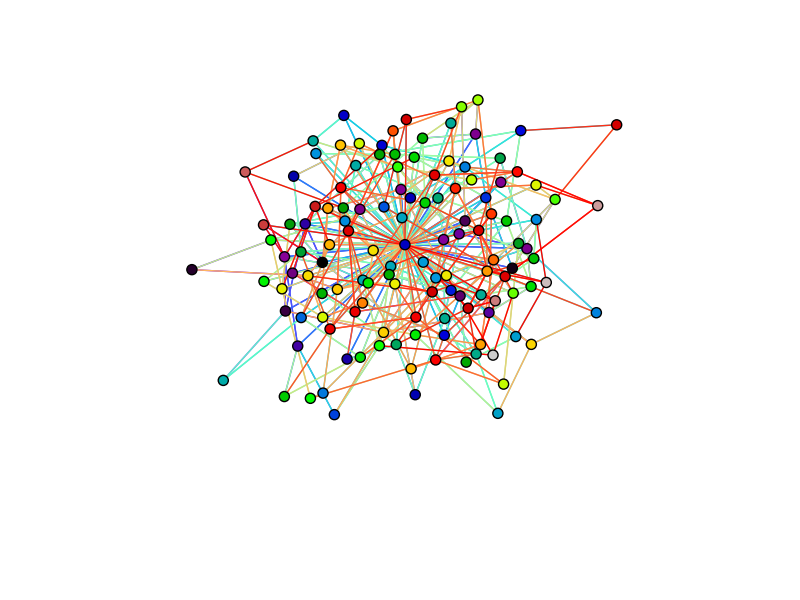
\includegraphics[width=0.8\columnwidth]{imagenes/exp5}
\caption{Grafo del experimento 5}
\label{fig:grafo5}
\end{center}
\end{figure}
\FloatBarrier

\subsubsection{Resultados del Experimento 5}
\par Tanto en In-Deg como en PageRank la p\'agina central es la primera en el ranking, pero en el caso de In-Deg la segunda es la p\'agina 36, que no es apuntada por la central.
En cambio en PageRank todas las primeras p\'aginas son apuntadas por la central, como es deseado.

\subsubsection{Experimento 6}
\par El experimento 6 consiste en juzgar la susceptibilidad de los m\'etodos a sucumbir bajo cierto tipo de ataque malicioso, donde una p\'agina crea otros sitios ''t\'iteres'' que apuntan a ella para aumentar su ranking.
Se espera que In-Deg sea m\'as vulnerable que PageRank, ya que estas p\'aginas maliciosas no son apuntadas por nadie 
(por lo que tienen un ranking inferior desde la perspectiva de PageRank, y por ende tendr\'an menor influencia en el orden final).
\par Se realizar\'an distintas iteraciones, manteniendo constante la cantidad de p\'aginas atacantes (en particular, 16 t\'iteres apuntando a un atacante), 
y variando la cantidad de p\'aginas normales, para ver como cambian los resultados al modificar la proporci\'on de p\'aginas atacantes y normales.
En las figuras \ref{fig:grafo6s64}, \ref{fig:grafo6s128} y \ref{fig:grafo6s256} se pueden observar los grafos que representan los distintos inputs.

\FloatBarrier
\begin{figure}[ht]
\subfigure[Grafo del experimento 6, para 64 p\'aginas normales]{
	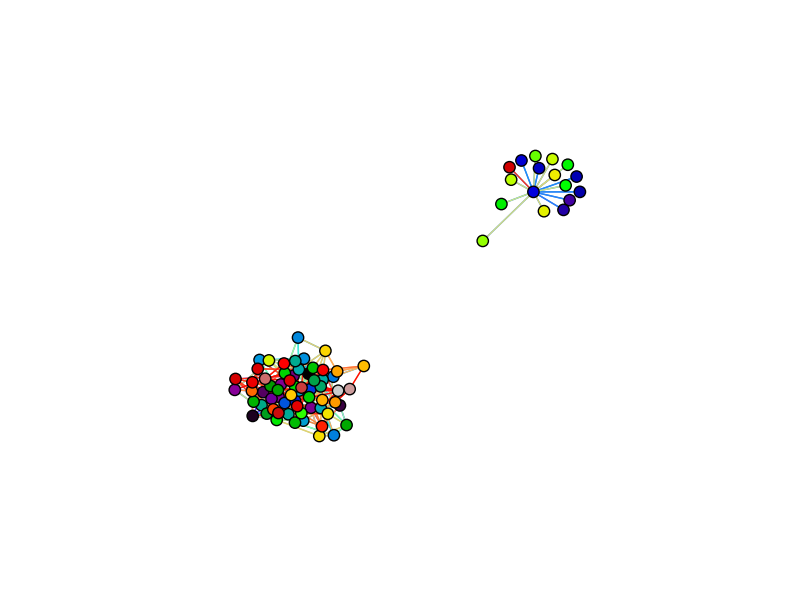
\includegraphics[width=0.45\columnwidth]{imagenes/exp6s64}
	\label{fig:grafo6s64}
}
\qquad
\subfigure[Grafo del experimento 6, para 128 p\'aginas normales]{
	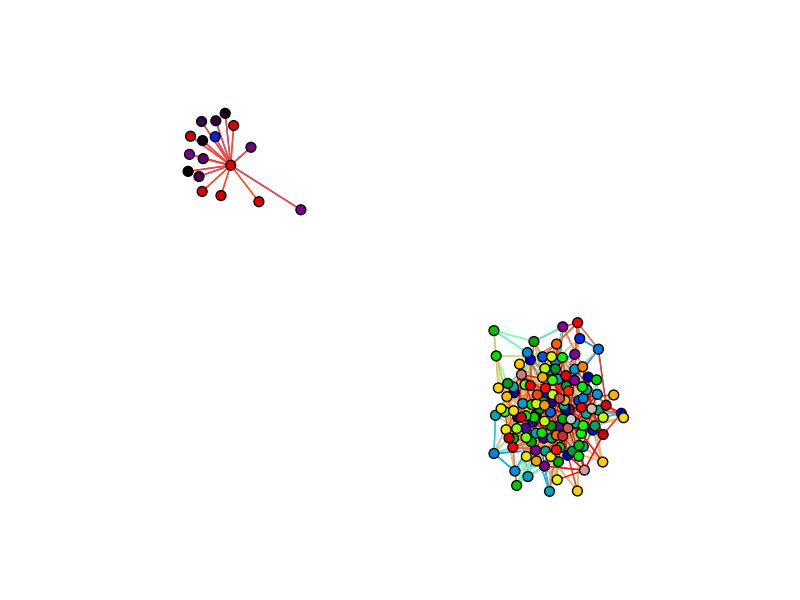
\includegraphics[width=0.45\columnwidth]{imagenes/exp6s128}
	\label{fig:grafo6s128}
}
\end{figure}

\begin{figure}[ht]
\subfigure[Grafo del experimento 6, para 256 p\'aginas normales]{
	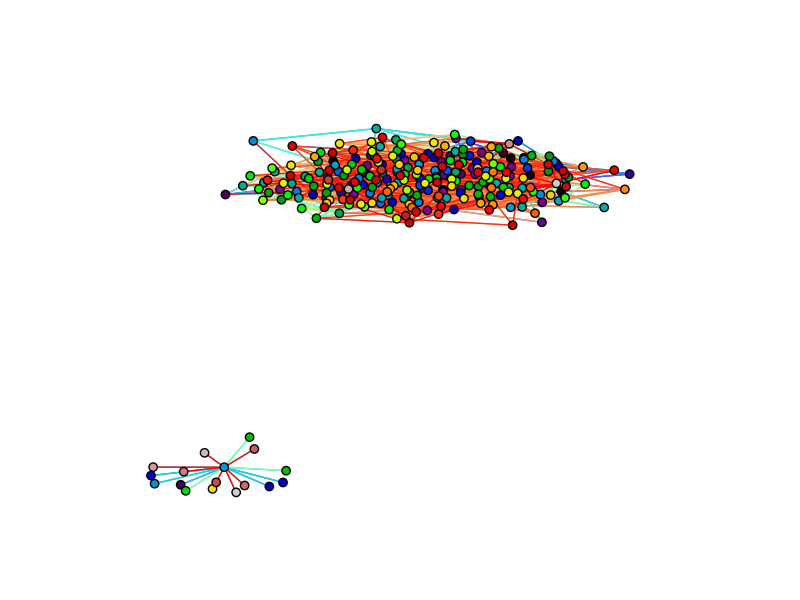
\includegraphics[width=0.45\columnwidth]{imagenes/exp6s256}
	\label{fig:grafo6s256}
}
\end{figure}

\FloatBarrier

\subsubsection{Resultados del Experimento 6}
\par En el caso de In-Deg, para las 3 entradas, la p\'agina atacante est\'a en la primera posici\'on del ranking.
En cambio, para PageRank, se encuentra en las posiciones 39, 77 y 153 (de un total de 81, 145 y 273, respectivamente).
Como se esperaba, PageRank es mucho menos vulnerable que In-Deg a este tipo de ataque.

\subsubsection{Experimento 7}
\par El s\'eptimo experimento busca juzgar la efectividad de nuestra variante de personalizaci\'on para el algoritmo PageRank.
Como entrada se utilizar\'a un grafo con 3 p\'aginas centrales (que se puede observar en la figura \ref{fig:grafo7}.
La idea es representar el resultado de un individuo buscando cierta expresi\'on en nuestro motor de b\'usqueda (por ejemplo ''Type of lambda expressions in C++11''),
y obteniendo como resultado ciertas p\'aginas, algunas de las cuales son ''centrales'' (como por ejemplo \textit{cplusplus.com}, \textit{cppreference.com} y \textit{stackoverflow.com})
y algunas son de menor importancia (por ejemplo blogs y otros sitios de ese tipo).
\par PageRank le asignar\'a un orden a estas p\'aginas, seguramente con las tres centrales arriba del ranking, pero cada usuario tendr\'a su propia preferencia de sitios.
Idealmente, el orden de los resultados de cada usuario tendr\'a en cuenta sus preferencias, y por ejemplo en el caso de las p\'aginas centrales, devolver\'a en primer lugar a su favorita.
Queremos comprobar que nuestro algoritmo de personalizaci\'on responde correctamente a un escenario de este tipo. 
Tambi\'en nos interesa ver como act\'ua frente a preferencias por sitios de menor importancia.
\par Realizaremos el mismo experimento con el mismo grafo de entrada previamente detallado, pero con diferentes entradas de personalizaci\'on.
En primer lugar, se utilizar\'a como control el resultado normal de PageRank; luego 3 historiales distintos donde el individuo prefiere cada una de las 3 p\'aginas centrales diferentes;
finalmente, un historial donde el usuario preferie mayoritariamente una p\'agina arbitraria.
Los historiales se encuentran detallados en los historiales 1, 2 y 3.
El par\'ametro \textit{''p''} de personalizaci\'on elegido es 0.5.

\FloatBarrier
\begin{figure}[ht]
\begin{center}
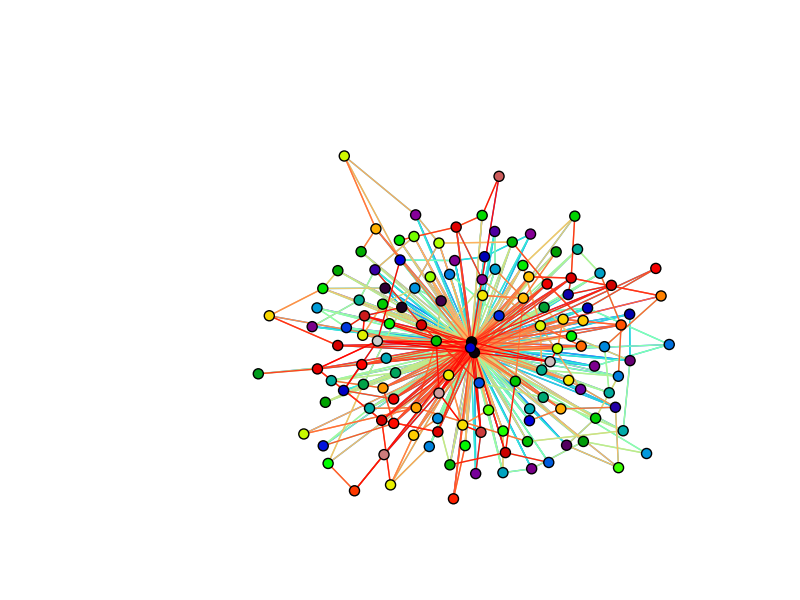
\includegraphics[width=0.8\columnwidth]{imagenes/exp7}
\caption{Grafo del experimento 7}
\label{fig:grafo7}
\end{center}
\end{figure}

\begin{multicols}{2}
\center
\begin{tabulary}{0.9\textwidth}{| c | c |}
\hline
\textbf{P\'agina} & \textbf{Cantidad de veces visitada} \\ \hline
5   & 19 \\ \hline
34  & 11 \\ \hline
80  & 12 \\ \hline
129 & 125\\ \hline
\end{tabulary}
\label{tab:in1}
Historial 1: Historial que prioritiza la p\'agina 129

\bigskip


\begin{tabulary}{0.9\textwidth}{| c | c |}
\hline
\textbf{P\'agina} & \textbf{Cantidad de veces visitada} \\ \hline
5   & 19 \\ \hline
34  & 11 \\ \hline
80  & 12 \\ \hline
130 & 125\\ \hline
\end{tabulary}
\label{tab:in2}
Historial 2: Historial que prioritiza la p\'agina 130

\bigskip


\begin{tabulary}{0.9\textwidth}{| c | c |}
\hline
\textbf{P\'agina} & \textbf{Cantidad de veces visitada} \\ \hline
5   & 19 \\ \hline
34  & 11 \\ \hline
80  & 12 \\ \hline
131 & 125\\ \hline
\end{tabulary}
\label{tab:in3}
Historial 3: Historial que prioritiza la p\'agina 131

\bigskip


\begin{tabulary}{0.9\textwidth}{| c | c |}
\hline
\textbf{P\'agina} & \textbf{Cantidad de veces visitada} \\ \hline
5   & 19 \\ \hline
34  & 11 \\ \hline
80  & 12 \\ \hline
124 & 125\\ \hline
\end{tabulary}
\label{tab:in4}
Historial 4: Historial que prioritiza la p\'agina 124

\bigskip

\end{multicols}

\subsubsection{Resultados del Experimento 7}


\begin{multicols}{2}
\center
\begin{tabulary}{0.9\textwidth}{| c | c |}
\hline
\textbf{Orden} & \textbf{P\'agina} \\ \hline
1   & 130\\ \hline
2   & 131\\ \hline
3   & 129\\ \hline
... & ---\\ \hline
46  & 5  \\ \hline
... & ---\\ \hline
67  & 124\\ \hline
\end{tabulary}
\label{tab:out1}
\linebreak
Tabla 1: Ranking de PageRank sin personalizaci\'on

\bigskip


\begin{tabulary}{0.9\textwidth}{| c | c |}
\hline
\textbf{Orden} & \textbf{P\'agina} \\ \hline
1   & 129\\ \hline
2   & 130\\ \hline
3   & 131\\ \hline
... & ---\\ \hline
9   & 5  \\ \hline
... & ---\\ \hline
\end{tabulary}
\label{tab:out2}
\linebreak
Tabla 2: Ranking de PageRank utilizando el historial que prioritiza la p\'agina 129

\bigskip


\begin{tabulary}{0.9\textwidth}{| c | c |}
\hline
\textbf{Orden} & \textbf{P\'agina} \\ \hline
1   & 130\\ \hline
2   & 131\\ \hline
3   & 129\\ \hline
... & ---\\ \hline
8   & 5  \\ \hline
... & ---\\ \hline
\end{tabulary}
\linebreak
Tabla 3: Ranking de PageRank utilizando el historial que prioritiza la p\'agina 130
\bigskip


\begin{tabulary}{0.9\textwidth}{| c | c |}
\hline
\textbf{Orden} & \textbf{P\'agina} \\ \hline
1   & 131\\ \hline
2   & 130\\ \hline
3   & 129\\ \hline
... & ---\\ \hline
15  & 5  \\ \hline
... & ---\\ \hline
\end{tabulary}
\label{tab:out4}
\linebreak
Tabla 4: Ranking de PageRank utilizando el historial que prioritiza la p\'agina 131

\columnbreak


\begin{tabulary}{0.9\textwidth}{| c | c |}
\hline
\textbf{Orden} & \textbf{P\'agina} \\ \hline
1   & 130\\ \hline
2   & 131\\ \hline
3   & 129\\ \hline
4   & 5  \\ \hline
... & ---\\ \hline
17  & 124\\ \hline
... & ---\\ \hline
\end{tabulary}
\label{tab:out5}
\linebreak
Tabla 5: Ranking de PageRank utilizando el historial que prioritiza la p\'agina 124, con $p = 0.5$

\bigskip


\begin{tabulary}{0.9\textwidth}{| c | c |}
\hline
\textbf{Orden} & \textbf{P\'agina} \\ \hline
1   & 5  \\ \hline
2   & 130\\ \hline
3   & 131\\ \hline
4   & 129\\ \hline
5   & 124\\ \hline
... & ---\\ \hline
\end{tabulary}
\label{tab:out6}
\linebreak
Tabla 6: Ranking de PageRank utilizando el historial que prioritiza la p\'agina 124, con $p = 0.95$

\bigskip


\begin{tabulary}{0.9\textwidth}{| c | c |}
\hline
\textbf{Orden} & \textbf{P\'agina} \\ \hline
1   & 130\\ \hline
2   & 131\\ \hline
3   & 129\\ \hline
4   & 5  \\ \hline
5   & 124\\ \hline
... & ---\\ \hline
\end{tabulary}
\label{tab:out7}
\linebreak
Tabla 7: Ranking de PageRank utilizando el historial que prioritiza la p\'agina 124, con $p = 0.75$ o $p = 0.85$

\bigskip

\end{multicols}

\par El resultado del control (que se puede observar en la tabla 1) efectivamente tiene a los 3 sitios centrales (en nuestro experimento, p\'aginas 129, 130 y 131) en las primeras 3 posiciones, en el orden 130, 131 y luego 129.
El sitio arbitrario (en este caso, el 124) se encuentra en el lugar 67 del ranking.
Las 3 iteraciones que prioritizan las distintas p\'aginas centrales (cuyos resultados se pueden encontrar en las tablas 2, 3 y 4) efectivamente tienen como resultado estos sitios en el primer lugar del ranking, que es lo deseado.
A su vez, la iteraci\'on (resultado en la tabla 5) que prioritiza la p\'agina arbitraria la tiene en el lugar 17.
Sin embargo, esta posici\'on es m\'as baja de la que esperamos debido a la alta prioridad que se le dio al sitio en el historial, 
lo que nos lleva a creer que \textit{''p''} en 0.5 puede ser demasiado sutil.
Realizamos nuevamente el experimento con \textit{''p''} en 0.85 y 0.95.
\par Con $p = 0.95$ (resultado en la tabla 6) la p\'agina 5 (que se encuentra en el historial de entrada, pero con frecuencia relativamente baja) sobrepasa a los sitios centrales.
Este resultado es excesivo, por lo que concluiremos que 0.95 es un valor demasiado alto para \textit{''p''}.
Tanto para $p = 0.85$ como para $p = 0.75$ (resultado en la tabla 7) la p\'agina 5 se encuentra en el cuarto lugar y la 124 en el quinto; por lo que concluimos que este es un rango aceptable para el par\'ametro de personalizaci\'on.

\newpage

\section{Resultados y Discusi\'on: Ligas Deportivas}
\par A continuaci\'on vamos a analizar resultados para el algoritmo GeM en el contexto de la Primera Divis\'on de la Liga Argentina de F\'utbol enfoc\'andonos en el ranking de equipos y experimentando sobre variaciones del ranking est\'andar, obtenci\'on del ranking mediante el m\'etodo GeM y m\'etodos alternatvos. Tomaremos como informaci\'on de entrada el campeonato 2015 hasta la fecha 26 inclusive. 
\bigskip

\par Contamos con el ranking oficial (est\'andar) de la liga que consta de ordenar los equipos por puntaje obtenido. Por cada partido ganado un equipo suma 3 puntos, por cada partido empatado obtiene tan solo 1, mientras que no obtiene puntos si fue derrotado. Como se puede ver el ranking no toma como informaci\'on relevante los goles. Mas adelante veremos que el m\'etodo GeM se basa fuertemente en los goles pero no diferencia entre victorias y derrotas tan notoriamente como si lo hace el ranking est\'andar.

\subsection{Experimento 1}
\par Como primer experimento vamos a comparar el ranking obtenido tras la aplicaci\'on del m\'etodo GeM y el ranking est\'andar tomando como entrada los resultados de todos los partidos hasta la fecha 26 inclusive. Creemos que van a notarse diferencias sobre todo por dos motivos:
\begin{itemize}
	\item El m\'etodo GeM no tiene en cuenta los empates, resultado que se da con frecuencia en el futbol argentino;
	\item El m\'etodo GeM solo se enfoca en los goles, mientras que el m\'etodo est\'andar solo se enfoca en quien gan\'o/empat\'o/perdi\'o.
\end{itemize}

\newpage

\subsubsection{Resultados del Experimento 1}

\begin{multicols}{2}
\center
\begin{tabulary}{0.45\textwidth}{| c | c | c | c | c |}
\hline
& \textbf{Equipo} & \textbf{Puntos} \\ \hline
1 & Boca Juniors & 58\\ \hline
2 & San Lorenzo & 54\\ \hline
3 & Rosario Central & 52\\ \hline
4 & Racing Club & 49\\ \hline
5 & River Plate & 48\\ \hline
6 & Independiente & 45\\ \hline
7 & Banfield & 43\\ \hline
8 & Belgrano & 43\\ \hline
9 & Estudiantes (LP) & 42\\ \hline
10 & Tigre & 42\\ \hline
11 & Quilmes & 39\\ \hline
12 & Lanús & 38\\ \hline
13 & Unión & 38\\ \hline
14 & Gimnasia y Esgrima (LP) & 37\\ \hline
15 & Newell's Old Boys & 33\\ \hline
16 & San Martín (SJ) & 32\\ \hline
17 & Aldosivi & 30\\ \hline
18 & Sarmiento & 30\\ \hline
19 & Argentinos Juniors & 29\\ \hline
20 & Olimpo & 29\\ \hline
21 & Temperley & 29\\ \hline
22 & Defensa y Justicia & 27\\ \hline
23 & Huracán & 26\\ \hline
24 & Vélez Sarsfield & 26\\ \hline
25 & Godoy Cruz & 25\\ \hline
26 & Colón & 24\\ \hline
27 & Arsenal & 23\\ \hline
28 & Atlético de Rafaela & 22\\ \hline
29 & Nueva Chicago & 17\\ \hline
30 & Crucero del Norte & 14\\ \hline
\end{tabulary}
\bigskip

Ranking mediante m\'etodo est\'andar.

\columnbreak

\begin{tabulary}{0.45\textwidth}{ | c | c | c |}
\hline
& \textbf{Equipo} & \textbf{Numero}\\ \hline
1 & Boca Juniors & 0.0860189\\ \hline
2 & Aldosivi & 0.0653536\\ \hline
3 & River Plate & 0.0634998\\ \hline
4 & San Lorenzo & 0.0620352\\ \hline
5 & Rosario Central & 0.0484731\\ \hline
6 & Racing Club & 0.0478783\\ \hline
7 & San Martín (SJ) & 0.0439558\\ \hline
8 & Quilmes & 0.0423821\\ \hline
9 & Newell's Old Boys & 0.0382332\\ \hline
10 & Vélez Sarsfield & 0.0376689\\ \hline
11 & Independiente & 0.0365646\\ \hline
12 & Belgrano & 0.0363978\\ \hline
13 & Gimnasia y Esgrima (LP) & 0.0335849\\ \hline
14 & Banfield & 0.0307372\\ \hline
15 & Estudiantes (LP) & 0.0295322\\ \hline
16 & Unión & 0.0288744\\ \hline
17 & Tigre & 0.0273356\\ \hline
18 & Sarmiento & 0.026108\\ \hline
19 & Huracán & 0.0246666\\ \hline
20 & Defensa y Justicia & 0.023737\\ \hline
21 & Lanús & 0.022729\\ \hline
22 & Olimpo & 0.0224689\\ \hline
23 & Arsenal & 0.0208702\\ \hline
24 & Godoy Cruz & 0.017516\\ \hline
25 & Temperley & 0.016045\\ \hline
26 & Crucero del Norte & 0.0160393\\ \hline
27 & Argentinos Juniors & 0.0153984\\ \hline
28 & Nueva Chicago & 0.0142318\\ \hline
29 & Atlético de Rafaela & 0.0113878\\ \hline
30 & Colón & 0.0102765\\ \hline
\end{tabulary}
\bigskip

Ranking mediante m\'etodo GeM.
\end{multicols}

\par En los resultados se puede observar que hay variaciones en las posiciones de los distintos equipos. Esto era de esperarse porque los m\'etodos usados se enfocan en distintos aspectos.
\bigskip

\par Vamos a analizar el caso particular de Aldosivi. En el ranking est\'andar se encuentra en la posici\'on 17, consecuencia de tan solo haber ganado 8 partidos y empatar 6 sobre 26 jugados. Mientras que en el ranking GeM se posiciona en el segundo lugar, veamos por qu\'e sucede esto. Recordemos que el m\'etodo GeM cuenta la diferencia de goles para con su rival en sus partidos ganados. Aldosivi, en los 8 partidos ganados no recibi\'o goles y convirti\'o 15. Cuenta entonces con una diferencia de goles importante, que lo posiciona en segundo lugar.

\par Con este claro ejemplo podemos ver la diferencia de enfoques de los dos m\'etodos. Creemos que para un deporte como el futbol el m\'etodo de GeM no est\'a bien formulado y no se enfoca en los resultados finales. Tal vez en otras ligas donde la diferencia de goles entre el ganador y el perdedor sea mayor (como la española o la alemana) y se den pocos empates pueda acercarse mas al m\'etodo est\'andar y/o competir con \'el sobre cu\'al deber\'ia ser el oficial.

\newpage

\subsection{Experimento 2}

\par Luego de analizar los resultados del experimento 1 queremos ver mas en detalle la influencia de los empates en el ranking obtenido por el m\'etodo GeM. Sabemos que al no tener en cuenta estos resultados nos alejamos del ranking est\'andar, pero queremos determinar si es factible que con alg\'un tipo de modificaci\'on podamos ajustarlo a un deporte con empates recurrentes (en este caso el f\'utbol).
\par Para tomar en consideraci\'on a los empates vamos a igualarlos a una victoria 1 a 0: ``empate = victoria por 1 a 0''. Sabemos que \'esto influye positivamente sobre los equipos con muchos empates, pero al darle un resultado favorable m\'inimo (1 a 0) creemos que no afectar\'a demasiado, manteniendo as\'i la base del enfoque del m\'etodo GeM y d\'andole cierta importancia a los empates.

\subsubsection{Resultados del Experimento 2}

\begin{figure}[ht]
\begin{center}
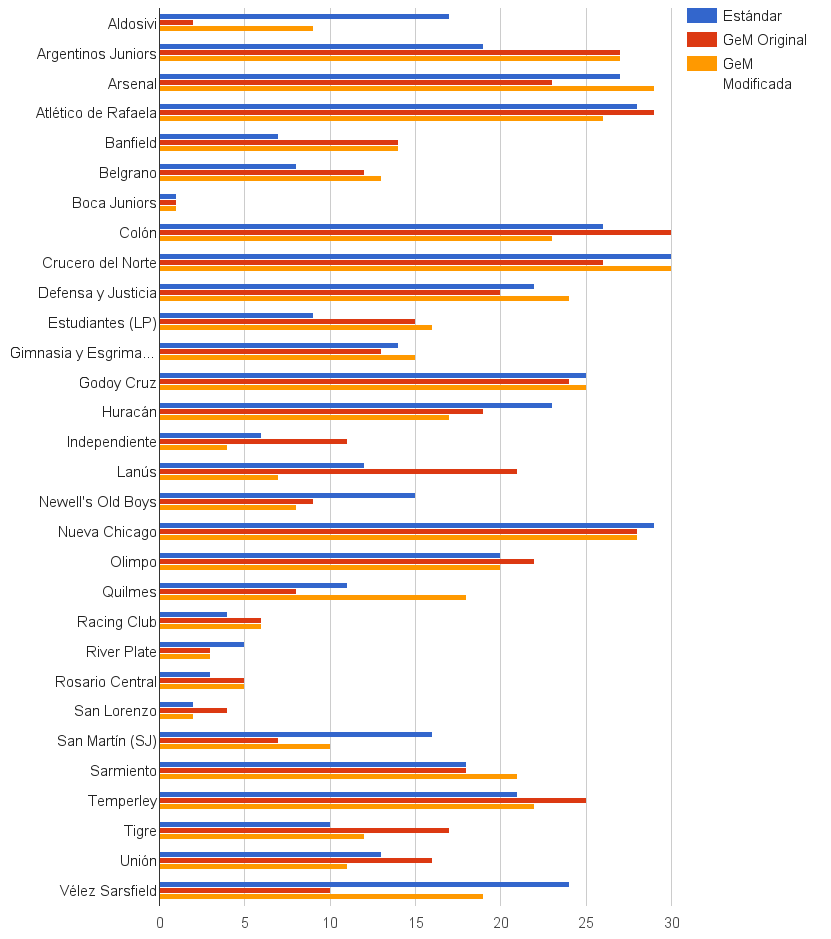
\includegraphics[width=0.7\columnwidth]{../src/experimentos/deportivos/2/experimento2.png}
\caption{Comparaciones de Rankings}
\end{center}
\end{figure}

\par En los resultados obtenidos vemos que la modificaci\'on del m\'etodo GeM gener\'o cambios en el posicionamiento de los equipos con empates en su historial. En algunos casos estos cambios lo alejaron de su posicionamiento en el ranking est\'andar mientras que en la mayor\'ia de los casos lo acercaron, d\'andole as\'i un cierto valor al empate que antes no era tenido en cuenta. Como nombramos antes, mantuvimos el enfoque del m\'etodo GeM pero le agregamos un pequeño valor a los empates que los gener\'o una tabla que creemos mas adecuada a la realidad del f\'utbol.

\newpage

\begin{multicols}{2}
\center
\begin{tabulary}{0.45\textwidth}{| c | c | c | c | c |}
\hline
& \textbf{Equipo} & \textbf{Puntos} \\ \hline
1 & Boca Juniors & 58\\ \hline
2 & San Lorenzo & 54\\ \hline
3 & Rosario Central & 52\\ \hline
4 & Racing Club & 49\\ \hline
5 & River Plate & 48\\ \hline
6 & Independiente & 45\\ \hline
7 & Banfield & 43\\ \hline
8 & Belgrano & 43\\ \hline
9 & Estudiantes (LP) & 42\\ \hline
10 & Tigre & 42\\ \hline
11 & Quilmes & 39\\ \hline
12 & Lanús & 38\\ \hline
13 & Unión & 38\\ \hline
14 & Gimnasia y Esgrima (LP) & 37\\ \hline
15 & Newell's Old Boys & 33\\ \hline
16 & San Martín (SJ) & 32\\ \hline
17 & Aldosivi & 30\\ \hline
18 & Sarmiento & 30\\ \hline
19 & Argentinos Juniors & 29\\ \hline
20 & Olimpo & 29\\ \hline
21 & Temperley & 29\\ \hline
22 & Defensa y Justicia & 27\\ \hline
23 & Huracán & 26\\ \hline
24 & Vélez Sarsfield & 26\\ \hline
25 & Godoy Cruz & 25\\ \hline
26 & Colón & 24\\ \hline
27 & Arsenal & 23\\ \hline
28 & Atlético de Rafaela & 22\\ \hline
29 & Nueva Chicago & 17\\ \hline
30 & Crucero del Norte & 14\\ \hline
\end{tabulary}
\bigskip

Ranking mediante m\'etodo est\'andar.

\columnbreak

\begin{tabulary}{0.4\textwidth}{ | c | c | c |}
\hline
& \textbf{Equipo} & \textbf{Numero}\\ \hline
1 & Boca Juniors & 0.0532173\\ \hline
2 & San Lorenzo & 0.0466695\\ \hline
3 & River Plate & 0.0466113\\ \hline
4 & Independiente & 0.0443246\\ \hline
5 & Rosario Central & 0.0436734\\ \hline
6 & Racing Club & 0.0391814\\ \hline
7 & Lanús & 0.0385408\\ \hline
8 & Newell's Old Boys & 0.0383858\\ \hline
9 & Aldosivi & 0.0381275\\ \hline
10 & San Martín (SJ) & 0.0370988\\ \hline
11 & Unión & 0.0370056\\ \hline
12 & Tigre & 0.0347199\\ \hline
13 & Belgrano & 0.0340198\\ \hline
14 & Banfield & 0.0340106\\ \hline
15 & Gimnasia y Esgrima (LP) & 0.0326107\\ \hline
16 & Estudiantes (LP) & 0.0319726\\ \hline
17 & Huracán & 0.0312592\\ \hline
18 & Quilmes & 0.0308084\\ \hline
19 & Vélez Sarsfield & 0.0306859\\ \hline
20 & Olimpo & 0.0304997\\ \hline
21 & Sarmiento & 0.0302557\\ \hline
22 & Temperley & 0.0277299\\ \hline
23 & Colón & 0.0267565\\ \hline
24 & Defensa y Justicia & 0.0262358\\ \hline
25 & Godoy Cruz & 0.024695\\ \hline
26 & Atlético de Rafaela & 0.024516\\ \hline
27 & Argentinos Juniors & 0.023696\\ \hline
28 & Nueva Chicago & 0.023149\\ \hline
29 & Arsenal & 0.0230411\\ \hline
30 & Crucero del Norte & 0.0165022\\ \hline
\end{tabulary}
\bigskip

Ranking obtenido por el m\'etodo GeM modificado.
\end{multicols}

\par Haciendo referencia al experimento 1, donde supimos comparar el ranking est\'andar del obtenido por el m\'etodo GeM, podemos sumar los resultados obtenidos con el m\'etodo GeM modificado. Notamos que las similitudes son mayores  a pesar de mantener distancia en los enfoques.

\newpage

\subsection{Experimento 3}

\par En este experimento analizaremos el impacto de la variación del parámetro $c$ sobre los resultados de rankings de competencias deportivas usando GeM. Vimos, por resultados anteriores, que aumentar el $c$ hace que el algoritmo se vuelva más lento, ya que tarda más en converger, pero devuelve resultados más justos. En este experimento nos centraremos en las diferencias entre los resultados y no en el tiempo de ejecución (ver Experimento 3 de la sección de resultados para Páginas Web).

\par Para llevar a cabo el experimento compararemos las tablas de posiciones obtenidas por cada equipo para ciertos valores de $c$, comparándolas con la posición actual en el ranking de la AFA.

\subsubsection{Resultados del Experimento 3}

\par Observemos la comparación entre las posiciones obtenidas por los equipos según cada $c$:

\begin{tabulary}{\textwidth}{| c | c | c | c | c | c | c |}
\hline						
\textbf{Pos. AFA} & \textbf{Equipo} & \textbf{c=0.85} & \textbf{c=0.65} & \textbf{c=0.45} & \textbf{c=0.25} & \textbf{c=0.00}\\ \hline
1 & Boca Juniors & 1 & 1 & 1 & 1 & 1 \\ \hline
2 & San Lorenzo & 4 & 3 & 2 & 2 & 1\\ \hline
3 & Rosario Central & 5 & 6 & 6 & 5 & 1\\ \hline
4 & Racing Club & 6 & 5 & 5 & 4 & 1\\ \hline
5 & River Plate & 3 & 2 & 3 & 3 & 1\\ \hline
6 & Independiente & 11 & 9 & 9 & 8 & 1\\ \hline
7 & Banfield & 14 & 14 & 13 & 13 & 1\\ \hline
8 & Belgrano & 12 & 11 & 10 & 9 & 1\\ \hline
9 & Estudiantes (LP) & 15 & 15 & 16 & 16 & 1\\ \hline
10 & Tigre & 17 & 15 & 15 & 14 & 1\\ \hline
11 & Quilmes & 8 & 7 & 7 & 7 & 1\\ \hline
12 & Lanús & 21 & 19 & 18 & 14 & 1\\ \hline
13 & Unión & 16 & 16 & 17 & 18 & 1\\ \hline
14 & Gimnasia y Esgrima (LP) & 13 & 13 & 12 & 12 & 1\\ \hline
15 & Newell's Old Boys & 9 & 10 & 11 & 11 & 1\\ \hline
16 & San Martín (SJ) & 7 & 8 & 8 & 10 & 1\\ \hline
17 & Aldosivi & 2 & 4 & 4 & 6 & 1\\ \hline
18 & Sarmiento & 18 & 18 & 19 & 19 & 1\\ \hline
19 & Argentinos Juniors & 27 & 26 & 25 & 25 & 1\\ \hline
20 & Olimpo & 22 & 23 & 23 & 23 & 1\\ \hline
21 & Temperley & 25 & 25 & 26 & 26 & 1\\ \hline
22 & Defensa y Justicia & 20 & 21 & 22 & 22 & 1\\ \hline
23 & Huracán & 19 & 20 & 20 & 20 & 1\\ \hline
24 & Vélez Sarsfield & 10 & 12 & 14 & 17 & 1\\ \hline
25 & Godoy Cruz & 24 & 24  & 24 & 24 & 1\\ \hline
26 & Colón & 30 & 30 & 30 & 30 & 1\\ \hline
27 & Arsenal & 23 & 22 & 21 & 21 & 1\\ \hline
28 & Atlético de Rafaela & 29 & 29 & 29 & 29 & 1\\ \hline
29 & Nueva Chicago & 28 & 28 & 28 & 28 & 1\\ \hline
30 & Crucero del Norte & 26 & 27 & 27 & 27 & 1\\ \hline
\end{tabulary}

\hspace{1cm}

\par Para las fechas del torneo de la AFA, no se ven grandes cambios en los resultados obtenidos variando el $c$ excepto en los casos de Lanús, y Vélez. Esto es una diferencia con el contexto de Páginas Web, ya que como las matrices de Markov de las competencias de fútbol no son esparsas (todos juegan contra todos), a diferencia del caso de las páginas web, no se nota tanto el impacto de la teletransportación. Sin embargo, como vimos en experimentos anteriores, debido a las diferencias de modelado del empate no podemos comparar cualitativamente si los resultados son más justos. 
\par Además, podemos ver que al disminuir el $c$ las distribuciones del vector estacionario se vuelven más equitativas, siendo el caso extremo $c = 0$, donde como se ve en la tabla, todos los equipos terminan en la misma posición.


